\chapter{Introducción al software científico\\ Introduction to scientific software}
\chaptermark{Intro al sw. científico \textreferencemark \ Intro to scientific sw.}
\epigraph{"Begin at the beginning", the King said, gravely, ''and go on till you came to the end; then stop"}{Lewis Carroll, Alice in Wonderland}
\begin{paracol}{2}
En la actualidad, el ordenador se ha convertido en una herramienta imprescindible para el trabajo de cualquier investigador científico. Su uso ha permitido realizar tareas que sin su ayuda resultarían sencillamente imposibles de acometer. Entre otras, distinguiremos las tres siguientes:
\begin{itemize}
\item Adquisición de datos de dispositivos experimentales.
\item Análisis y tratamiento de datos experimentales. \index{Datos, análisis}
\item Cálculo Ciéntifico.
\end{itemize}
\switchcolumn
Computers have become an essential tool in the daily work of every Scientific researcher. They are used for doing tasks that could not be carried out without their help. We can point out the following tasks, among others:
 \begin{itemize}
\item Data acquisition from experimental devices.
\item Experimental data analysis and processing. \index{Data, analysis}
\item Scientific computing.
\end{itemize}     


\switchcolumn
La primera de éstas tareas queda fuera de los contenidos de esta asignatura. Su objetivo es emplear el ordenador para recoger datos automáticamente de los sensores empleados en un dispositivo experimental. El procedimiento habitual es emplear dispositivos electrónicos que traducen las lecturas de un sensor (un termómetro, un manómetro, un caudalímetro, una cámara etc.) a un voltaje. El voltaje es digitalizado, es decir, convertido a una secuencia de ceros y unos, y almacenado en un ordenador para su posterior análisis o/y directamente monitorizado, es decir, mostrado en la pantalla del ordenador. En muchos casos el ordenador es a su vez capaz de interactuar con el dispositivo experimental: iniciar o detener un experimento, regular las condiciones en que se realiza, disparar alarmas si se producen errores, etc.

\switchcolumn
The first of these tasks is beyond the scope of this course. It aims to use the computer to get data automatically from the sensors attached to an experimental device. Usually, data supplied by a sensor (a thermometer, a manometer, a flow meter, an optical Camera, etc.) are converted to voltages by some electronic device. Then, the voltages are digitalized ---i.e., converted to a sequence of zeros and ones---  and stored in a computer for later analysis. Also, they can be shown (monitored) on a computer screen. In many cases, the computer can also interact with the experimental device: start or stop an experiment, control the experimental conditions, trigger an alarm in case of error, etc.          

\switchcolumn
De este modo, el investigador científico, queda dispensado de la tarea de adquirir por sí mismo los datos experimentales. Tarea que en algunos casos resultaría imposible, por ejemplo si necesita medir muchas variables a la vez o si debe medirlas a gran ritmo; y en la que, en general, es relativamente fácil cometer errores.

\switchcolumn
In this way, the scientific researcher is released from getting the experimental data by himself. A task that could sometimes be impossible to do. For instance, when he needs to measure many variables simultaneously or when the measurements must be taken quickly. Besides, it is easy to make mistakes when the measurements are manually taken.     

\switchcolumn
El análisis y tratamiento de datos experimentales, constituye una tarea fundamental dentro del trabajo de investigación científica. Los ordenadores permiten realizar dichas tareas, de una forma eficiente y segura con cantidades de datos que resultarían imposibles de manejar hace 50 años. Como veremos más adelante, una simple hoja de cálculo puede ahorrarnos una cuantas horas de cálculos tediosos. El análisis estadístico de un conjunto de datos experimentales, el cálculo --la estimación-- de los errores experimentales cometidos, la posterior regresión de los datos obtenidos a una función matemática que permita establecer una ley o al menos una relación entre los datos obtenidos, formar parte del trabajo cotidiano del investigador, virtualmente en todos los campos de la ciencia.

\switchcolumn
Experimental data analysis and processing are fundamental tasks in scientific work. The computers carry out such tasks efficiently and safely, working with data amounts that were impossible to deal with fifty years ago. As we shall see later, a simple data sheet can save us many hours of tedious calculations. Statistical analysis of experimental data, Estimation of experimental errors, and regression of data to a mathematical function allows us to establish a law or at least find a relationship among the data. All these are part of researchers' daily work, virtually in any field of science.  
     
\switchcolumn
Por último el cálculo. \index{Cálculo numérico} Cabría decir que constituye el núcleo del trabajo de investigación. El científico trata de explicar la realidad que le rodea, mediante el empleo de una descripción matemática. Dicha descripción suele tomar la forma de un modelo matemático más o menos complejo. La validez de un modelo está ligada a que sea capaz de reproducir los resultados experimentales obtenidos del fenómeno que pretende explicar. Si el modelo es bueno será capaz de obtener mediante cálculo unos resultados similares a los obtenido mediante el experimento. De este modo, el modelo queda validado y es posible emplearlo para predecir cómo se comportará el sistema objeto de estudio en otras condiciones.

\switchcolumn
Lastly, computing \index[eng]{Scientific computing}. It can be said that scientific computing is the kernel of scientific work. The researcher tries to explain the real world using a mathematical description. Such a description usually takes the form of a mathematical model, which can be more or less complex. A model is valid because it can reproduce the same results as the original experiment, which the model tries to explain. If the model is good enough, it can be obtained by computing similar results from the experiment. Then, the model becomes tested and can be used to forecast the system's behaviour under study in many different conditions.     
\end{paracol}

%\section{Introducción a los computadores.\\ Introduction to computers.} \index{Computador} \index{Ordenador}

\begin{paracol}{2}
\section[Introducción a los computadores.]{Introducción a los com\-putadores.\sectionmark{Intro  a los computadores \textreferencemark \ Intro to computers}}
\sectionmark{Intro  a los computadores \textreferencemark \ Intro to computers}
Más o menos todos estamos familiarizados con lo que es un computador, los encontramos a diario continuamente  y, de hecho, hay muchos aspectos de nuestra vida actual que serían inimaginables sin los computadores.  En términos muy generales, podemos definir un computador como una máquina que es capaz de recibir instrucciones y realizar operaciones (cálculos) a partir de las instrucciones recibidas. Precisamente es la capacidad de recibir instrucciones lo que hace del ordenador una herramienta versátil; según las instrucciones recibidas y de acuerdo también a sus posibilidades como máquina,  el ordenador puede realizar tareas muy distintas, entre las que cabe destacar como más generales, las siguientes:
\begin{itemize}
\item Procesamiento de datos 
\item Almacenamiento de datos
\item Transferencias de datos entre el computador y el exterior
\item Control de las anteriores operaciones
\end{itemize}

\switchcolumn
\section{Introduction to compu\- ters.}
Everybody is somehow familiar with computers. We find them daily, and we depend on them in such a way that our current lives would be unimaginable without them. In general, a computer can be defined as a machine able to get instructions and data and use the instructions to perform calculations with the data. The capacity to get instruction makes the computer a versatile tool; according to the instruction received and the specific machine capacity, the computer can carry out very different tasks. Among them, we can highlight the following:
\begin{itemize}
\item data processing
\item data storing
\item data transfer between the computer and the outside.
\item Control of these operations just listed.
\end{itemize}    

\switchcolumn
El computador se diseña para realizar funciones generales que se especifican cuando se programa. La programación es la que concreta las tareas que efectivamente realiza un ordenador concreto.

\switchcolumn
The computer is designed to perform general functions which are specified when the computer is programmed. Programming is the way to define the tasks the computer will carry out. 

\end{paracol}
 


\begin{paracol}{2}
\subsection{Niveles de descripción de un ordenador.}
La figura \ref{fig:nivel} muestra un modelo general de un computador descrito por niveles. Cada nivel, supone y se apoya en el nivel anterior. 
\begin{figure}[ht]
	\centering
		%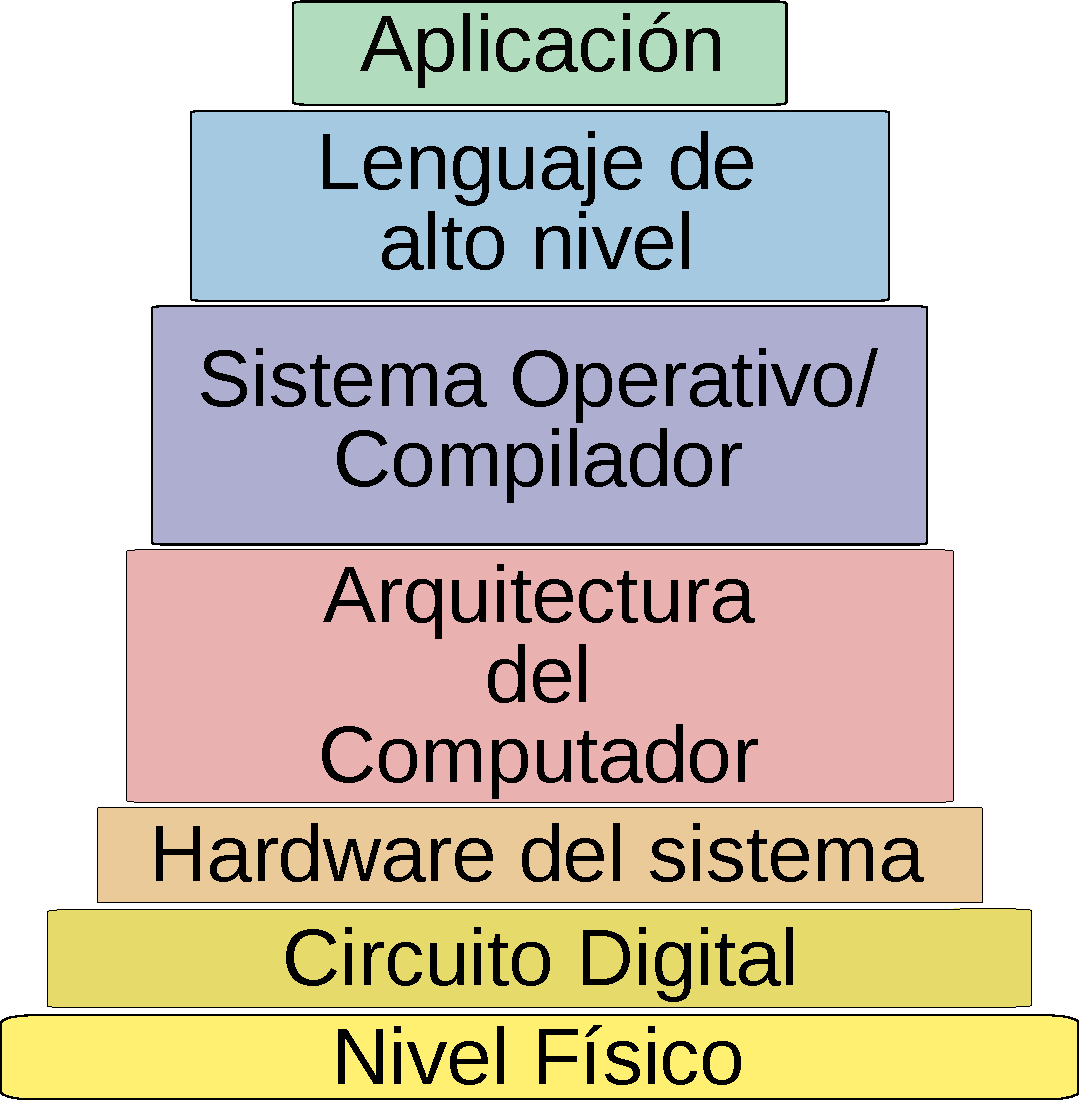
\includegraphics[width=10cm]{nivel_descripcion.pdf}
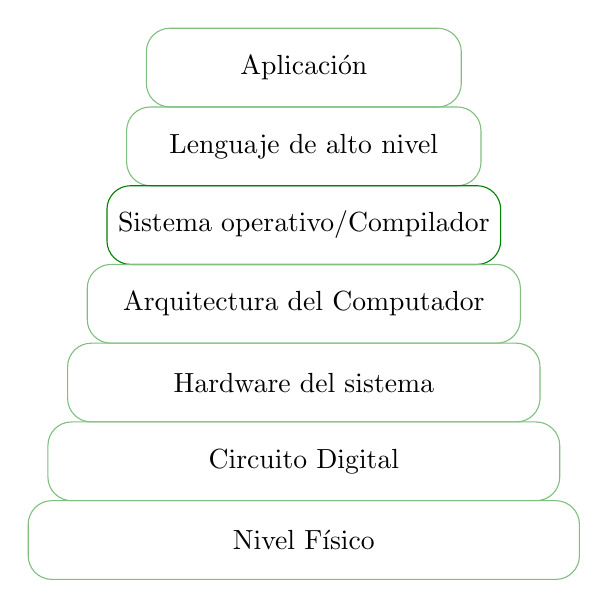
\begin{tikzpicture}
\draw (0,0)node[rectangle,minimum width=4cm, minimum height=1cm ,rounded corners=3mm,draw = green!50!black!50]{Aplicación};
\draw (0,-1)node[rectangle,minimum width=4.5cm, minimum height=1cm ,rounded corners=3mm,draw = green!50!black!50]{Lenguaje de alto nivel};
\draw (0,-2)node[rectangle,minimum width=5cm, minimum height=1cm ,rounded corners=3mm,draw = green!50!black!]{Sistema operativo/Compilador};
\draw (0,-3)node[rectangle,minimum width=5.5cm, minimum height=1cm ,rounded corners=3mm,draw = green!50!black!50]{Arquitectura del Computador};
\draw (0,-4)node[rectangle,minimum width=6cm, minimum height=1cm ,rounded corners=3mm,draw = green!50!black!50]{Hardware del sistema};
\draw (0,-5)node[rectangle,minimum width=6.5cm, minimum height=1cm ,rounded corners=3mm,draw = green!50!black!50]{Circuito Digital};
\draw (0,-6)node[rectangle,minimum width=7cm, minimum height=1cm ,rounded corners=3mm,draw = green!50!black!50]{Nivel Físico};
\end{tikzpicture}
	\caption{Descripción por niveles de un computador}
	\label{fig:nivel}
\end{figure}
\switchcolumn
Figure \ref{fig:nivele} shows a general computer layout described by levels. Each level lays and assume the previous level. 
\begin{figure}[ht]
	\centering
		%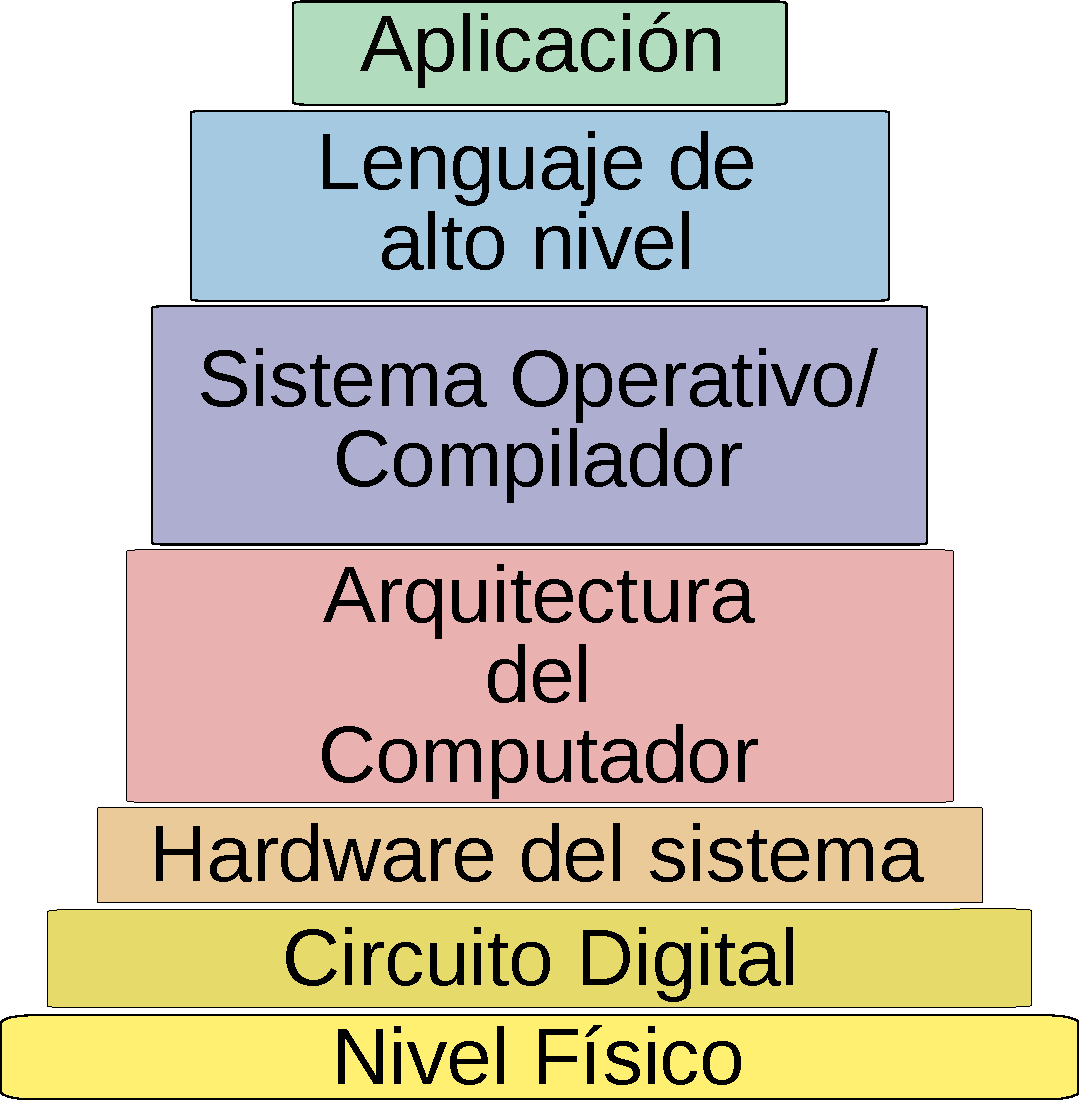
\includegraphics[width=10cm]{nivel_descripcion.pdf}
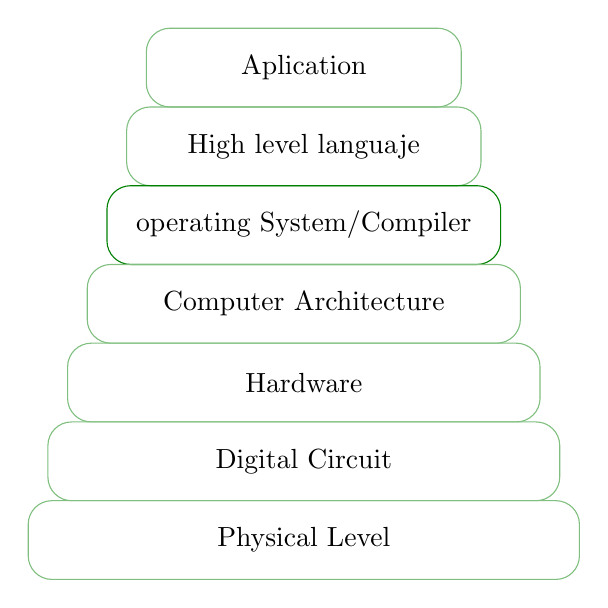
\begin{tikzpicture}
\draw (0,0)node[rectangle,minimum width=4cm, minimum height=1cm ,rounded corners=3mm,draw = green!50!black!50]{Aplication};
\draw (0,-1)node[rectangle,minimum width=4.5cm, minimum height=1cm ,rounded corners=3mm,draw = green!50!black!50]{High level languaje};
\draw (0,-2)node[rectangle,minimum width=5cm, minimum height=1cm ,rounded corners=3mm,draw = green!50!black!]{operating System/Compiler};
\draw (0,-3)node[rectangle,minimum width=5.5cm, minimum height=1cm ,rounded corners=3mm,draw = green!50!black!50]{Computer Architecture};
\draw (0,-4)node[rectangle,minimum width=6cm, minimum height=1cm ,rounded corners=3mm,draw = green!50!black!50]{Hardware};
\draw (0,-5)node[rectangle,minimum width=6.5cm, minimum height=1cm ,rounded corners=3mm,draw = green!50!black!50]{Digital Circuit};
\draw (0,-6)node[rectangle,minimum width=7cm, minimum height=1cm ,rounded corners=3mm,draw = green!50!black!50]{Physical Level};
\end{tikzpicture}
	\renewcommand{\figurename}{Figure}
	\caption{Computer level description}
	\label{fig:nivele}
\end{figure}
\switchcolumn
\begin{enumerate}
\item \textbf{Nivel Físico.} Constituye la base del \emph{hardware} del computador. Está constituido por los componentes electrónicos básicos, diodos, transistores, resistencias, etc.  En un computador moderno, no es posible separar o tan siquiera observar dichos componentes: Se han fabricado directamente sobre un cristal semiconductor, y forman parte de un dispositivo electrónico conocido con el nombre de circuito integrado.

\item \textbf{Circuito Digital.}
Los componentes del nivel físico se agrupan formando circuitos digitales, (En nuestro caso circuitos digitales integrados). Los circuitos digitales trabajan solo con dos niveles de tensión ($V_1, V_0$) lo que permite emplearlos para establecer relaciones lógicas:\\ $V_1$=verdadero, $V_2$=falso. Estas relaciones lógicas establecidas empleando los valores de la tensión de los circuitos digitales constituyen el soporte de todos los cálculos que el computador puede realizar.

\item \textbf{Organización Hardware del sistema.}\index{Computador ! \emph{hardware}} 
Los circuitos digitales integrados se agrupan y organizan para formar el \emph{Hardware} del ordenador.  Los módulos básicos que constituyen el \emph{Hardware} son la unidad central de procesos (CPU), La unidad de memoria y las unidades de entrada y salida de datos. Dichos componentes están conectados entre sí mediante un bus, que transfiere datos de una unidad a otra.

\item \textbf{Arquitectura del computador.} \index{Computador ! arquitectura}
La arquitectura define cómo trabaja el computador. Por tanto, está estrechamente relacionada con la organización hardware del sistema, pero opera a un nivel de abstracción superior. Establece cómo se accede a los registros de memoria, arbitra el uso de los buses que comunican unos componentes con otros, y regula el trabajo de la CPU.  

Sobre la arquitectura se establece el lenguaje básico en el que trabaja el ordenador, conocido cómo lenguaje máquina. Es un lenguaje que emplea todavía niveles lógicos binarios (ceros o unos) y por tanto no demasiado apto para ser interpretado por los seres humanos. Este lenguaje permite al ordenador realizar operaciones básicas como copiar el contenido de un registro de memoria en otro, sumar el contenido de dos registros de memoria, etc. 

El lenguaje máquina es adecuado para los computadores, pero no para los humanos, por eso, los fabricantes suministran junto con el computador un repertorio básico de instrucciones que su máquina puede entender y realizar en un lenguaje algo más asequible. Se trata del lenguaje ensamblador. Los comandos de éste lenguaje son fácilmente traducibles en una o varias instrucciones de lenguaje máquina.   Aún así se trata de un lenguaje en el que programar directamente resulta una tarea tediosa y proclive a cometer errores. 

\item \textbf{Compiladores y Sistemas Operativos} \index{Sistema operativo} \index{Compilador}
Los Compiladores constituyen un tipo de programas especiales que permiten convertir un conjunto de instrucciones, escritas en un lenguaje de alto nivel en lenguaje máquina. El programador escribe sus instrucciones en un fichero de texto normal, perfectamente legible para el ser humano, y el compilador convierte las instrucciones contenidas en dicho fichero en secuencias binarias comprensibles por la máquina.

Los computadores primitivos solo eran capaces de ejecutar un programa a la vez. A medida que se fueron fabricando ordenadores mas sofisticados, surgió la idea de crear programas que se encargaran de las tareas básicas: gestionar el flujo de información, manejar periféricos, etc. Estos programas reciben el nombre de sistemas operativos. Los computadores modernos cargan al arrancar un sistema operativo que controla la ejecución del resto de las aplicaciones. Ejemplos de sistemas operativos son DOS (Disk Operating System), Unix y su versión para ordenadores personales Linux.

\item \textbf{Lenguajes de alto nivel.} \index{Programación! lenguajes}
Los lenguajes de alto nivel están pensados para facilitar la tarea del programador, desentendiéndose de los detalles de implementación del hardware del ordenador.  Están compuestos por un conjunto de comandos y unas reglas sintácticas, que permiten describir las instrucciones para el computador en forma de texto.

De una manera muy general, se pueden dividir los lenguajes de alto nivel en lenguajes compilados y lenguajes interpretados. Los lenguajes compilados emplean un compilador para convertir los comandos del lenguaje de alto nivel en lenguaje máquina. Ejemplos de lenguajes compilados son C , C++ y Fortran. Los lenguajes interpretados a diferencia de los anteriores no se traducen a lenguaje máquina antes de ejecutarse. Si no que utilizan otro programa --el interprete-- que va leyendo los comandos del lenguaje y convirtiéndolos en instrucciones máquina a la vez que el programa se va ejecutando. Ejemplos de programas interpretado son Basic, Python y Java.

\item \textbf{Aplicaciones.} \index{Programación! aplicaciones} Se suele entender por aplicaciones programas orientados a tareas específicas, disponibles para un usuario final. Habitualmente se trata de programas escritos en un lenguaje de alto nivel y presentados en un formato fácilmente comprensible para quien los usa.

Existen multitud de aplicaciones, entre las más conocidas cabe incluir los navegadores para Internet, como Explorer, Mocilla o Google Crome, los editores de texto, como Word, las hojas de cálculo como Excel o los clientes de correo como Outlook. En realidad, la lista de aplicaciones disponibles en el mercado sería interminable. 
\end{enumerate}

\switchcolumn
\subsection{Computer description levels.}
\begin{enumerate}
\item \textbf{Physical Level.} It's the ground of the computer hardware. Basic electronic components, diodes, transistors, resistances, etc, make it up. In a modern computer, it is impossible to split or even to watch such components: they are built directly in a semiconductor Crystal and part\; of an electronic device Known as \emph{integrated circuit}.

\item \textbf{Digital Circuit.}
Physical level components are grouped, forming digital circuits. (In our case, Integrated digital circuits). They work with only two voltage levels ($V_1, V_0$). This allows us to use them for defining logical relationships: $V_1$=true, $V_2$=false. This logical relationship obtained using two voltage levels of digital circuits is, in turn, the basis for every computing the computer can carry out.

\item \textbf{Computer Hardware organisation.}\index[eng]{Computer ! \emph{hardware}} 
Digital circuits are grouped and organized to build up the computer Hardware. Basic hardware modules are the central processing unit(CPU), the memory unit and the input and output units. These components are connected by a bus, which transfers data from one unit to another.

\item \textbf{Computer Architecture.} \index[eng]{Computer ! architecture}
The architecture defines how the computer works. Thus, it is highly related to the hardware organization of the system; bit architecture works at a higher abstraction level. It defines how to get access to the memory register, arbitrate the use of the buses with links to the different components and regulates the CPU work.   
 
The primary language the computer works with is established according to its architecture. This primary language is called Machine language. It still uses binary logical levels (zeros and ones), so it is unsuitable for being understood by human beings. The computer uses machine language to perform basic operations such as copying the content from one memory register to another, adding the contents of two memory registers, etc.     

Machine language is suitable for computers but not for human beings. Thus, manufacturers supply the computer with a basic repertory of instructions that their machine can understand and carry out, written in a more accessible language. It is known as assembler language. The commands of this language are accessible to translate to one or several machine language instructions. Writing code right in assembler language is tedious and prone to mistakes.     
   
\item \textbf{Compilers y operating Systems} \index[eng]{operating system} \index[eng]{Compiler}
Compilers are special programs that allow us to translate instructions written in a high-level language into machine language. The programmer writes instructions in plain text, readable for a human being. Then, the compiler translates the file's contents into binary sentences that the machine can interpret.
       
Early computers were only able to run a program at a time. As new and more sophisticated computers were built, it arises the idea of making programs which were able to take over the basic tasks:
Managing the information flow, dealing with peripheral devices, etc. These programs are called operating systems. Modern computers load an operating system at the boot time, which controls the running of the remaining programs. Some examples of operating systems are DOS (Disk Operating System), UNIX and the UNIX version for personal computers LINUX.       

\item \textbf{High level languages} \index[eng]{Programming! languages}
High-level languages are intended to make the programmer's work easier, ignoring the hardware implementation details.   They comprise a set of commands and syntactic rules, allowing the programmer to describe computer instruction in plain text.

Generally, High-level languages can be divided into compiled and interpreted languages. Compiled languages employ a compiler to traduce the command from the high-level language to machine language. Some examples are C, C++ and FORTRAN. On the contrary, interpreted languages do not translate to machine language. They use a second program known as the interpreter. While a program in the interpreted language is running, the interpreter reads the program commands one by one and translates them to machine language. Examples of interpreted languages are BASIC, Python or Java.  


\item \textbf{Programmes.} \index[eng]{Programming! Programmes} 
A Programme is a piece of code intended to perform specific tasks. They are available to the final users of the computer. Usually, programs are written using a high-level language and are user-friendly, i.e. they have an interface that is easy to use.

There are many different kinds of programs, according to their purpose. We can find Internet web browsers like Google Chrome, Mozilla or Explorer, text editors like Word, Emacs or Latex.    
E-mail clients (Mail User Agents) like Outlook or Mozilla Thunderbird. The list of available programs would be endless. 
\end{enumerate}

\end{paracol}



\begin{paracol}{2}
\subsection{El modelo de computador de Von Neumann} \index{Von Neumann}

Los computadores modernos siguen, en lineas generales, el modelo propuesto por Von Neumann.  La figura \ref{fig:vonn} muestra un esquema de dicho modelo. 

\begin{figure}[ht]
	\centering
	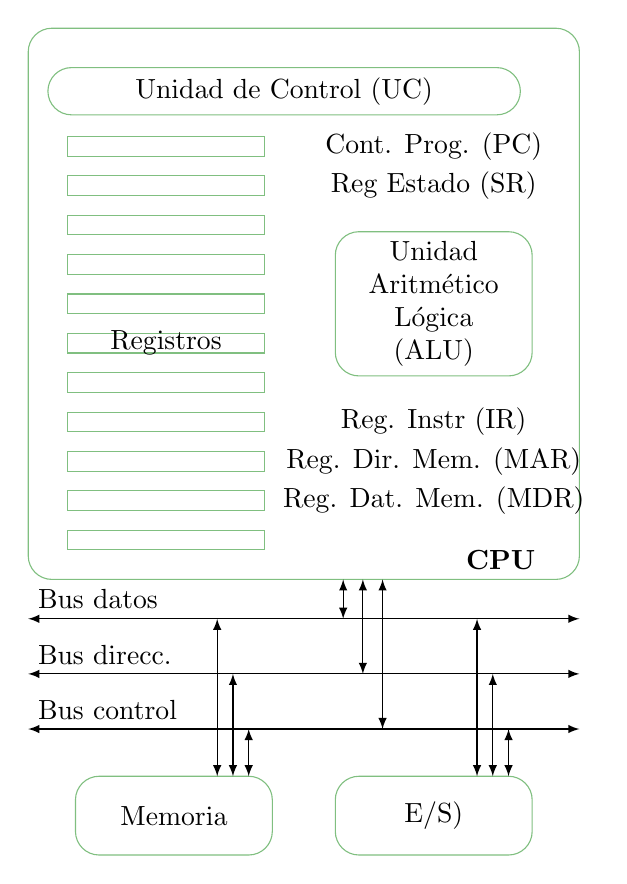
\begin{tikzpicture}
\draw (0,0)node[rectangle,minimum width=7cm, minimum height=7cm ,rounded corners=3mm,draw = green!50!black!50]{};
\draw (-0.25,2.7)node[rectangle,minimum width=6cm, minimum height=0.6cm ,rounded corners=3mm,draw = green!50!black!50]{Unidad de Control (UC)};
\draw (-1.75,2)node[rectangle,minimum width=2.5cm, minimum height=0.25cm ,draw = green!50!black!50]{};
\draw (-1.75,1.5)node[rectangle,minimum width=2.5cm, minimum height=0.25cm , draw = green!50!black!50]{};
\draw (-1.75,1)node[rectangle,minimum width=2.5cm, minimum height=0.25cm, draw = green!50!black!50]{};
\draw (-1.75,0.5)node[rectangle,minimum width=2.5cm, minimum height=0.25cm ,draw = green!50!black!50]{};
\draw (-1.75,0)node[rectangle,minimum width=2.5cm, minimum height=0.25cm ,draw = green!50!black!50]{};
\draw (-1.75,-0.5)node[rectangle,minimum width=2.5cm,minimum height=0.25cm ,draw = green!50!black!50]{};
\draw (-1.75,-0.5)node[rectangle,minimum width=2.5cm,minimum height=0.25cm]{Registros};
\draw (-1.75,-1)node[rectangle,minimum width=2.5cm, minimum height=0.25cm,,draw = green!50!black!50]{};
\draw (-1.75,-1.5)node[rectangle,minimum width=2.5cm, minimum height=0.25cm , draw = green!50!black!50]{};
\draw (-1.75,-2)node[rectangle,minimum width=2.5cm, minimum height=0.25cm, draw = green!50!black!50]{};
\draw (-1.75,-2.5)node[rectangle,minimum width=2.5cm, minimum height=0.25cm ,draw = green!50!black!50]{};
\draw (-1.75,-3)node[rectangle,minimum width=2.5cm, minimum height=0.25cm ,draw = green!50!black!50]{};
\draw (1.65,2)node[rectangle,minimum width=2.5cm, minimum height=0.25cm]{Cont. Prog. (PC)};
\draw (1.65,1.5)node[rectangle,minimum width=2.5cm, minimum height=0.25cm]{Reg Estado (SR)};
\draw (1.65,0)node[rectangle,minimum width=2.5cm, minimum height=0.25cm, rounded corners=3mm ,draw = green!50!black!50,align=center]{Unidad \\ Aritmético \\ Lógica\\ (ALU)};
\draw (1.65,-1.5)node[rectangle,minimum width=2.5cm, minimum height=0.25cm]{Reg. Instr (IR)};
\draw (1.65,-2)node[rectangle,minimum width=2.5cm, minimum height=0.25cm]{Reg. Dir. Mem. (MAR)};
\draw (1.65,-2.5)node[rectangle,minimum width=2.5cm, minimum height=0.25cm]{Reg. Dat. Mem. (MDR)};
\draw (2.5,-3.25)node[rectangle,minimum width=2.5cm, minimum height=0.25cm]{\textbf{CPU}};
\draw[latex-latex](0.5,-3.5)--(0.5,-4);
\draw[latex-latex](0.75,-3.5)--(0.75,-4.7);
\draw[latex-latex](1,-3.5)--(1,-5.4);
\draw[latex-latex](-3.5,-4)node[anchor=south west]{Bus datos}--(3.5,-4);
\draw[latex-latex](-3.5,-4.7)node[anchor=south west]{Bus direcc.}--(3.5,-4.7);
\draw[latex-latex](-3.5,-5.4)node[anchor=south west]{Bus control}--(3.5,-5.4);

\draw (-1.65,-6.5)node[rectangle,minimum width=2.5cm, minimum height=1cm, rounded corners=3mm ,draw = green!50!black!50,align=center]{Memoria};
\draw (1.65,-6.5)node[rectangle,minimum width=2.5cm, minimum height=1cm, rounded corners=3mm ,draw = green!50!black!50,align=center]{E/S)};
\draw[latex-latex](-0.7,-5.4)--(-0.7,-6);
\draw[latex-latex](-0.9,-4.7)--(-0.9,-6);
\draw[latex-latex](-1.1,-4)--(-1.1,-6);

\draw[latex-latex](2.6,-5.4)--(2.6,-6);
\draw[latex-latex](2.4,-4.7)--(2.4,-6);
\draw[latex-latex](2.2,-4)--(2.2,-6);
\end{tikzpicture}	
	\caption{Modelo de Von Neumann}
	\label{fig:vonn}
\end{figure}

\switchcolumn
\subsection{The Von Neumann's computer model} \index[eng]{Von Neumann}
Modern computers generally follow the model proposed by Von Neumann. Figure \ref{fig:vonne} shows a schematic view of Von Neumann's model.  
\begin{figure}[ht]
	\centering
	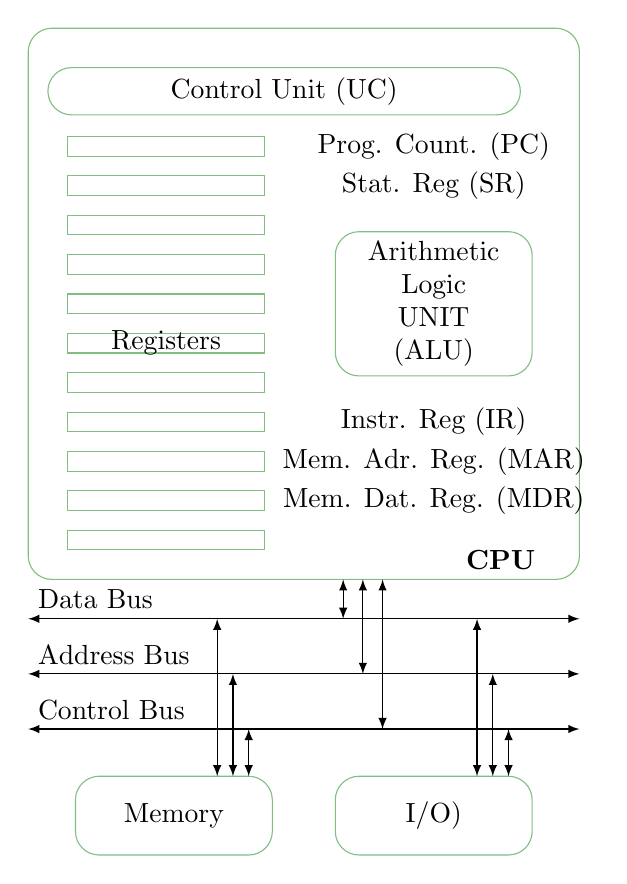
\begin{tikzpicture}
\draw (0,0)node[rectangle,minimum width=7cm, minimum height=7cm ,rounded corners=3mm,draw = green!50!black!50]{};
\draw (-0.25,2.7)node[rectangle,minimum width=6cm, minimum height=0.6cm ,rounded corners=3mm,draw = green!50!black!50]{Control Unit (UC)};
\draw (-1.75,2)node[rectangle,minimum width=2.5cm, minimum height=0.25cm ,draw = green!50!black!50]{};
\draw (-1.75,1.5)node[rectangle,minimum width=2.5cm, minimum height=0.25cm , draw = green!50!black!50]{};
\draw (-1.75,1)node[rectangle,minimum width=2.5cm, minimum height=0.25cm, draw = green!50!black!50]{};
\draw (-1.75,0.5)node[rectangle,minimum width=2.5cm, minimum height=0.25cm ,draw = green!50!black!50]{};
\draw (-1.75,0)node[rectangle,minimum width=2.5cm, minimum height=0.25cm ,draw = green!50!black!50]{};
\draw (-1.75,-0.5)node[rectangle,minimum width=2.5cm,minimum height=0.25cm ,draw = green!50!black!50]{};
\draw (-1.75,-0.5)node[rectangle,minimum width=2.5cm,minimum height=0.25cm]{Registers};
\draw (-1.75,-1)node[rectangle,minimum width=2.5cm, minimum height=0.25cm,,draw = green!50!black!50]{};
\draw (-1.75,-1.5)node[rectangle,minimum width=2.5cm, minimum height=0.25cm , draw = green!50!black!50]{};
\draw (-1.75,-2)node[rectangle,minimum width=2.5cm, minimum height=0.25cm, draw = green!50!black!50]{};
\draw (-1.75,-2.5)node[rectangle,minimum width=2.5cm, minimum height=0.25cm ,draw = green!50!black!50]{};
\draw (-1.75,-3)node[rectangle,minimum width=2.5cm, minimum height=0.25cm ,draw = green!50!black!50]{};
\draw (1.65,2)node[rectangle,minimum width=2.5cm, minimum height=0.25cm]{Prog. Count. (PC)};
\draw (1.65,1.5)node[rectangle,minimum width=2.5cm, minimum height=0.25cm]{Stat. Reg (SR)};
\draw (1.65,0)node[rectangle,minimum width=2.5cm, minimum height=0.25cm, rounded corners=3mm ,draw = green!50!black!50,align=center]{Arithmetic \\ Logic\\ UNIT\\ (ALU)};
\draw (1.65,-1.5)node[rectangle,minimum width=2.5cm, minimum height=0.25cm]{Instr. Reg (IR)};
\draw (1.65,-2)node[rectangle,minimum width=2.5cm, minimum height=0.25cm]{Mem. Adr. Reg. (MAR)};
\draw (1.65,-2.5)node[rectangle,minimum width=2.5cm, minimum height=0.25cm]{Mem. Dat. Reg. (MDR)};
\draw (2.5,-3.25)node[rectangle,minimum width=2.5cm, minimum height=0.25cm]{\textbf{CPU}};
\draw[latex-latex](0.5,-3.5)--(0.5,-4);
\draw[latex-latex](0.75,-3.5)--(0.75,-4.7);
\draw[latex-latex](1,-3.5)--(1,-5.4);
\draw[latex-latex](-3.5,-4)node[anchor=south west]{Data Bus}--(3.5,-4);
\draw[latex-latex](-3.5,-4.7)node[anchor=south west]{Address Bus }--(3.5,-4.7);
\draw[latex-latex](-3.5,-5.4)node[anchor=south west]{Control Bus}--(3.5,-5.4);

\draw (-1.65,-6.5)node[rectangle,minimum width=2.5cm, minimum height=1cm, rounded corners=3mm ,draw = green!50!black!50,align=center]{Memory};
\draw (1.65,-6.5)node[rectangle,minimum width=2.5cm, minimum height=1cm, rounded corners=3mm ,draw = green!50!black!50,align=center]{I/O)};
\draw[latex-latex](-0.7,-5.4)--(-0.7,-6);
\draw[latex-latex](-0.9,-4.7)--(-0.9,-6);
\draw[latex-latex](-1.1,-4)--(-1.1,-6);

\draw[latex-latex](2.6,-5.4)--(2.6,-6);
\draw[latex-latex](2.4,-4.7)--(2.4,-6);
\draw[latex-latex](2.2,-4)--(2.2,-6);
\end{tikzpicture}	
	\caption{Von Neumann's model}
	\label{fig:vonne}
\end{figure}

\switchcolumn
En el modelo de Von Newman se pueden  distinguir tres módulos básicos y una serie de elementos de interconexión.  Los módulos básicos son: 

\begin{itemize}
\item \textbf{La Unidad Central de Procesos.} CPU \index{CPU} (\emph{Central process unit)}) , esta unidad constituye el núcleo en el que el ordenador realiza las operaciones. 

Dentro de la CPU pueden a su vez distinguirse las siguientes partes:

\begin{itemize}

\item La unidad de proceso ó ruta de datos: Está formada por La Unidad Aritmético Lógica (ALU), \index{ALU} capaz de realizar las operaciones aritméticas y lógicas que indican las instrucciones del programa. En general las ALUs se construyen para realizar aritmética entre enteros, y realizar las operaciones lógicas básicas del algebra de Boole (AND, OR, etc). Habitualmente, las operaciones para números no enteros, representados en \emph{punto flotante} se suelen realizar empleando un procesador específico que se conoce con el nombre de Coprocesador matemático. La velocidad de procesamiento suele medirse en millones de operaciones por segundo (MIPS) o millones de operaciones en punto flotante por segundo (MFLOPS).

\item El banco de registros: Conjunto de registros en los que se almacenan los datos con los que trabaja la ALU y los resultados obtenidos.
 
\item La unidad de control (UC) o ruta de control: se encarga de buscar las instrucciones en la memoria principal y guardarlas en el registro de instrucciones, las decodifica, las ejecuta empleando la ALU, guarda los resultados en el registro de datos, y guarda las condiciones derivadas de la operación realizada en el registro de estado.  El registro de datos de memoria, contiene los datos que se están leyendo de la memoria principal o van a escribirse en la misma. El registro de direcciones de memoria, guarda la dirección de la memoria principal a las que esta accediendo la ALU, para leer o escribir. El contador del programa, también conocido como puntero de instrucciones, es un registro que guarda la posición en la que se encuentra la CPU dentro de la secuencia de instrucciones de un programa.
\end{itemize}
 

\item \textbf{La unidad de memoria.} Se trata de la memoria principal o primaria del computador.  Está dividida en bloques de memoria que se identifican mediante una dirección. La CPU tiene acceso directo a dichos bloques de memoria.

La unidad elemental de información digital es el bit \index{bit} (0,1). La capacidad de almacenamiento de datos se mide en Bytes \index{Byte} y en sus múltiplos, calculados siempre como potencias de 2:

\begin{align} \nonumber
1\  Byte = &\ 8\ bits\ &\  \\ \nonumber
1\  KB  = &\ 2^{10}\ bits=1024\ B&\ \\  \nonumber
1\  MB = &\ 2^{20}\ bits=1024\ KB&\ \\  \nonumber
1\  GB = &\ 2^{30}\ bits &\ \\  \nonumber
1\  TB  = &\ 2^{40}\ bits\ &\
\end{align} 

\item \textbf{Unidad de Entrada/Salida.} Transfiere información entre el computador y los dispositivos periféricos.
\end{itemize}

Los elementos de interconexión se conocen con el nombre de \emph{Buses}. Se pueden distinguir tres: En bus de datos, por el que se transfieren datos entre la CPU y la memoria ó la unidad de entrada/salida. El bus de direcciones, par especificar una dirección de memoria o del registro de E/S. Y el bus de Control, por el que se envían señales de control, tales como la señal de reloj, la señal de control de lectura/escrituras entre otras.

\switchcolumn
Von Neuman's model has been divided into three basic models and several interconnection elements. The basic modules are: 

\begin{itemize}
\item \textbf{The Central Processing Unity.} CPU \index{CPU} This Unity is the kernel where the computer performs operations. 

Inside the CPU, it is possible to difference the following parts:

\begin{itemize}

\item The processing unit or data router comprises the Arithmetic Logic Unit (ALU), \index{ALU}. The ALU can perform the arithmetical and logical operations described in the program instructions. They are built to perform arithmetic between integer numbers and the basic Boole's algebra logical operations (AND, OR, etc). Non-integer numbers are usually represented using a unique format called \emph{floating point representation}. Operations between floating point numbers are performed using a specific processor known as a coprocessor. The processing speed is measured in millions of instructions per second (MIPS) or millions of floating point operations per second (MFLOPS).

\item The register bank: A set of registers for storing the data ALU is working with and the results of ALU operations.
 
\item The control unit (UC) or control route: It fetches the instructions from the main memory and stores them in the instruction register. It also decoded the instructions, executed them using the ALUs, and stored the results in the data register. Once the operation is finished, the UC stores the conditions derived from the operation in the state register. The memory data register holds the data read from the main memory or those ready to be written there. Memory Address register holds the main memory address the ALU is accessing for writing or reading. The programme counter, or the instruction pointer, is a special register. It stores the current position at which the CPU is located inside a program instructions sequence.    
\end{itemize}
 

\item \textbf{Memory Unit} It is the main or primary memory of the computer. It is divided into memory blocks. Each memory block is identified by its address. The CPU has direct access to memory blocks.

The elemental unit of digital information is the \emph{bit} \index{bit}(0,1). Data storing capacity is gauged in Bytes \index{Byte} and multiples of Byte, represented as powers of two:

\begin{align} \nonumber
1\  Byte = &\ 8\ bits\ &\  \\ \nonumber
1\  KB  = &\ 2^{10}\ bits=1024\ B&\ \\  \nonumber
1\  MB = &\ 2^{20}\ bits=1024\ KB&\ \\  \nonumber
1\  GB = &\ 2^{30}\ bits &\ \\  \nonumber
1\  TB  = &\ 2^{40}\ bits\ &\
\end{align} 

\item \textbf{Input/Output Unit}. This unit transfers information between the computer and the peripheral devices.
\end{itemize}

The interconnection elements are called \emph{Buses}. We can define three: the data bus transfers data between the CPU and the main memory or the input/output unity. The address bus is used for transmitting a memory address or an input/output unit. The control bus for sending control signals, such as the clock signal and the reading/writing control signal, among others.     
\end{paracol} 


\begin{paracol}{2}
\subsection{Representación binaria} \index{Base 2}
Veamos con algo más de detalle, cómo representa la información un computador. Como se explicó anteriormente, La electrónica que constituye la parte física del ordenador, trabaja con dos niveles de voltaje. Esto permite definir dos estados, --alto, bajo-- que pueden representarse dos símbolos  $0$ y $1$. Habitualmente, empleamos $10$ símbolos: \\${0,1,2,3,4,5,6,7,8,9}$, es decir, empleamos una representación decimal. Cuando queremos representar números mayores que nueve, dado que hemos agotado el número de dígitos disponibles, lo que hacemos es combinarlos, agrupando cantidades de diez en diez. Así por ejemplo, el numero $16$, representa seis unidades más un grupo de diez unidades y el número $462$ representa dos unidades más seis grupos de diez unidades más cuatro grupos de 10 grupos de 10 unidades.  Matemáticamente, esto es equivalentes a emplear sumas de dígitos por potencias de diez:
\switchcolumn
\subsection{Binary coding} \index[eng]{Base 2}

Let's see in more detail how a computer represents the information. As described before, the electronic stuff represents the computer's physical part. It works with two voltage levels, which can be associated with two states ---high and low--- and, in turn, these levels can define two symbols, $0$ and $1$. Usually, we employ $10$ symbols (digits):\\ ${0,1,2,3,4,5,6,7,8,9}$, i.e. we use a \emph{decimal} representation. Whenever we want to represent a number greater than nine, we combine several symbols, gathering quantities in groups of ten because we have exhausted the ten available digits. So, for instance,  the number $16$ represents six units plus a group of ten units, and the number $462$ represents two units plus six groups of ten units, plus four groups of ten groups of 10 units. In mathematics, this is equal to using sums of products of digits by powers of ten:       

\end{paracol}
\begin{equation*}
13024 = 1\times10^4+3\times10^3+0\times10^2+2\times10^1+4\times10^0 
\end{equation*}

\begin{paracol}{2}
Si recorremos los dígitos que componen el número de izquierda derecha, cada uno de ellos representa una potencia de diez superior, porque cada uno representa la cantidad de grupos de 10 grupos, de grupos ... de diez grupos de unidades. Esto hace que potencialmente podamos representar cantidades tan grandes como queramos, empleando tan solo diez símbolos. Esta representación, a la que estamos habituados recibe el nombre de representación en base 10 \index{Base 10}. Pero no es la única posible.

\switchcolumn
If we look at the digits that compose the number from left to right, each one represents an upper power of ten, i.e., each represents the number of groups of ten groups of groups ... of ten groups of unities. This means we can represent amounts as significant as we wish, using only ten symbols. We are used to this numerical representation, which is known as a decimal representation or representation in base $10$. But it is not the only one.   

\switchcolumn
Volvamos a la representación empleada por el computador. En este caso solo tenemos dos símbolos distintos el $0$ y el $1$. Si queremos emplear una representación análoga a la representación en base diez, deberemos agrupar ahora las cantidad en grupos de dos. Así los únicos números que admiten ser representados con un solo dígito son el uno y el cero. Para representar el número dos, necesitamos agrupar: tendremos $0$ unidades y $1$ grupo de dos, con lo que la representación del número dos en base dos será $10$. Para representar el número tres, tendremos una unidad más un grupo de dos, por lo que la representación será $11$, y así sucesivamente. Matemáticamente esto es equivalente emplear sumas de dígitos por potencias de 2:

\switchcolumn
Returning to the computer's numerical representation, we have only two digits: $0$ and $1$. If we want to define a representation that resembles the base $10$ representation, we must now gather the quantities in groups of two. So, the number two is represented in base $2$ as $10$. To represent the number three, we have a group of two plus one unit $11$. In mathematics, this is equal to using sums of products of digits by powers of two;               
\end{paracol}

\begin{equation*}
10110 = 1\times2^4+0\times2^3+1\times2^2+1\times2^1+0\times2^0 
\end{equation*}
\begin{paracol}{2}
Esta representación recibe el nombre de representación binaria o en base 2.
\index{Conversión! binario a decimal}La expansión de un número representado en binario en potencias de 2, nos da un método directo de obtener su representación decimal. Así, para el ejemplo anterior, si calculamos las potencias de dos y sumamos los resultados obtenemos:
\switchcolumn
This representation is known as binary coding. \index{Conversion! binary to decimal} If we expand the binary encoding of a number as powers of two, we obtain a direct way to obtain its decimal representation. For instance, If we take the last example, calculate the power of two and add the results we obtain,
\end{paracol}
  \begin{equation*} 1\times2^4+0\times2^3+1\times2^2+1\times2^1+0\times2^0=16+0+4+2+0=22 
\end{equation*}
\begin{paracol}{2}
que es la representación en base 10 del número binario $10110$.
\switchcolumn
which is the representation on base 10 for the binary number $10110$
\end{paracol}
\begin{paracol}{2}
Para números no enteros, la representación tanto en decimal como en binario, se extiende de modo natural empleando potencias negativas de 10 y de 2 respectivamente. Así,
\switchcolumn
For non-integer numbers, decimal and binary representations of a number extend straightforwardly using the negative powers of 10 and 2, respectively. So,   
\end{paracol}
\begin{equation} \nonumber
835.41 = 8\times10^2+3\times10^1+5\times10^0+4\times10^{-1}+1\times10^{-2} 
\end{equation}
\begin{paracol}{2}
y para un número en binario,
\switchcolumn
and for a binary number,
\end{paracol}

\begin{equation} \nonumber
101.01 = 1\times2^2+0\times2^1+1\times2^0+0\times2^{-1}+1\times2^{-2} 
\end{equation}

De nuevo, basta calcular el término de la derecha de la expresión anterior para obtener la representación decimal del número $101.01$.

\index{Conversión! decimal a binario. números enteros}¿Cómo transformar la representación de un número de decimal a binario? De nuevo nos da la clave la representación en sumas de productos de dígitos por potencias de dos. Empecemos por el caso de un número entero. Supongamos un número D, representado en decimal. Queremos expandirlo en una suma de potencias de dos. Si dividimos el número por 2, podríamos representarlo cómo:
 
\begin{equation*}
\label{eq:1}
D=2\cdot C_1+R_1
\end{equation*}

donde $C_1$ representa el cociente de la división y $R_1$ el resto. Como estamos dividiendo por dos, el resto solo puede valer cero o uno. Supongamos ahora que volvemos a dividir el cociente obtenido por dos,

 \begin{equation*}
 \label{eq:2}
C_1=2\cdot C_2+R_2 \
\end{equation*}

Si sustituimos el valor obtenido para $C_1$ en la ecuación inicial obtenemos,   
\begin{equation*}
D=2\cdot(2\cdot C_2+R_2)+R_1= 2^2\cdot C_2+R_2\cdot 2^1+R_1\cdot 2^0 
\end{equation*}

Si volvemos a dividir el nuevo cociente obtenido $C_2$ por dos, y volvemos a sustituir,

 \begin{align*}
C_2&=2\cdot C_3+R_3 \\
D&=2^2\cdot(2\cdot C_3+R_3)+R_2\cdot 2^1+R_1\cdot 2^0=2^3\cdot C_3+R_3\cdot 2^2 +R_2\cdot 2^1+R_1\cdot 2^0
\end{align*}

Supongamos que tras repetir este proceso $n$ veces, obtenemos un conciente $C_n=1$. Lógicamente no tiene sentido seguir dividiendo ya que a partir de este punto, cualquier división posterior que hagamos nos dará cociente $0$ y resto igual a $C_n$. Por tanto, 

 \begin{align*}
D&=1\cdot 2^n+R_n\cdot 2^{n-1}\cdots +R_3\cdot 2^2 +R_2\cdot 2^1+R_1\cdot 2^0
\end{align*}

La expresión obtenida, coincide precisamente con la expansión en potencias de dos del número binario $1R_n \cdots R_3R_2R_1$.


Como ejemplo,podemos obtener la representación en binario del número $234$, empleando el método descrito: vamos dividiendo el número y los cocientes sucesivos entre dos, hasta obtener un cociente igual a uno y a continuación, construimos la representación binaria del número colocando por orden, de derecha a izquierda.  los restos  obtenidos de las sucesivas divisiones y añadiendo un uno más a la izquierda de la cifra construida con los restos:

\begin{table}[h]
\begin{tabular}{|r|r|r|r|}
Dividendo& &Cociente $\div 2$&Resto\\
\hline
234& &117&0\\
117& &58&1\\
58& &29&0\\
29& &14&1\\
14& &7&0\\
7& &3&1\\
3& &1&1
\end{tabular}
\end{table}
 
 Por tanto, la representación en binario de 234 es 11101010.
 
\index{Conversión! decimal a binario, números no entero}Supongamos ahora un número no entero, representado en decimal, de la forma $0,d$ . Si lo multiplicamos por dos:

\begin{equation}
E_1,d_1=0,d\cdot 2
\end{equation}
Donde $E_1$ representa la parte entera y $d_1$ la parte decimal del número calculado.
Podemos entonces representar $0,d$ como,
\begin{equation}
\label{eq:5}
0,d=(E_1,d_1)\cdot 2^{-1}=E_1\cdot 2^{-1}+0,d_1\cdot 2^{-1}
\end{equation}  

Si volvemos a multiplicar $0,d_1$ por dos,

\begin{equation}
E_2,d_2 = 0,d_1\cdot 2
\end{equation}

\begin{equation}
0,d_1=E_2\cdot 2^{-1}+0,d_2\cdot 2^{-1}
\end{equation}  

y sustituyendo en \ref{eq:5}

\begin{equation}
0,d=E_1\cdot 2^{-1}+E_2\cdot 2^{-2}+0,d_2\cdot 2^{-2}
\end{equation}

¿Hasta cuando repetir el proceso? En principio hasta que obtengamos un valor cero para la parte decimal, $0,d_n=0$. Pero esta condición puede no cumplirse nunca. Puede darse el caso --de hecho es lo más probable-- de que un número que tiene una representación exacta en decimal, no la tenga en binario. El criterio para detener el proceso será entonces obtener un determinado número de decimales o bien seguir el proceso hasta que la parte decimal obtenida vuelva a repetirse. Puesto que los ordenadores tienen un tamaño de registro limitado, también está limitado el número de dígitos con el que pueden representar un número decimal. Por eso, lo habitual será truncar el número asumiendo el error que se comete al proceder así.  De este modo, obtenemos la expansión del número original en potencias de dos,

\begin{equation}
0,d\cdot 2=E_1\cdot 2^{-1}+E_2\cdot 2^{-2}+\cdots+ E_n\cdot 2^{-3}+\cdots
\end{equation} 

Donde los valores $E_1\cdots E_n$ son precisamente los dígitos correspondientes a la representación del número en binario: $0.E_1E_2\cdots E_n$. (Es trivial comprobar que solo pueden valer $0$ ó $1$).


Veamos un ejemplo de cada caso, obteniendo la representación binaria del número $0,625$, que tiene representación exacta, y la del número $0,626$, que no la tiene. En este segundo caso, calcularemos una representación aproximada, tomando 8 decimales.

\begin{table}[h]
\begin{tabular}{|r|r|r|r|r r|r|r|r|r|}
P decimal& &$\times 2$& P entera& &&P decimal& &$\times 2$& P entera\\
\cline{1-4}
\cline{7-10}
0,625& &1,25&1& &&0,623& &1,246&1\\
0,25  & &0,5  &0& &&0,246& &0,492&0\\
0,5    & &1,0  &1& &&0,492& &0,984&0\\
         & &       &  & &&0,984& &1,968&1\\
         & &       &  & &&0,968& &1,936&1\\
         & &       &  & &&0,936& &1,872&1\\
         & &       &  & &&0.872& &1.744&1\\
         & &       &  & &&0.744& &1.488&1\\
\end{tabular}
\end{table}

Para construir la representación binaria del primero de los números, nos basta tomar las partes enteras obtenidas, por orden, de derecha a izquierda y añadir un $0$ y la coma decimal a la izquierda. Por tanto  la representación binaria de $0,625$ es $0,101$.  Si expandimos su valor en potencias de dos, volvemos a recuperar el número original en su representación decimal.

 En el segundo caso, la representación binaria, tomando nueve decimales de $0,623$ es $0.10011111$. Podemos calcular el error que cometemos al despreciar el resto de los decimales, volviendo a convertir el resultado obtenido a su representación en base diez,

 \begin{equation*}
0\cdot 2^{0}+1\cdot 2^{-1}+0\cdot 2^{-2}+ 0\cdot 2^{-3}+1\cdot 2^{-4}+1\cdot 2^{-5}+ 1\cdot 2^{-6}+1\cdot 2^{-7}+1\cdot 2^{-8}=0,62109375
\end{equation*} 

El error cometido es, en este caso: $\text{Error}=0,623-0,62109375=0,00190625$.
  
 \section{Aplicaciones de Software Científico}
Dentro del mundo de las aplicaciones, merecen una mención aparte las dedicadas al cálculo científico, por su conexión con la asignatura. 

Es posible emplear lenguajes de alto nivel para construir rutinas y programas que permitan resolver directamente un determinado problema de cálculo. En este sentido, el lenguaje FORTRAN se ha empleado durante años para ese fin, y todavía sigue empleándose en muchas disciplinas científicas y de la Ingeniería.  Sin embargo, hay muchos aspectos no triviales del cálculo con un computador, que obligarían al científico que tuviera que programar sus propios programas a ser a la vez un experto en computadores.  Por esta razón, se han ido desarrollando aplicaciones específicas para cálculo científico que permiten al investigador centrarse en la resolución de su problema y no en el desarrollo de la herramienta adecuada para resolverlo.  
 
En algunos casos, se trata de aplicaciones a medida, relacionadas directamente con algún área científica concreta. En otros, consisten en paquetes de funciones específicos para realizar de forma eficiente determinados cálculos, como por ejemplo
el paquete SPSS para cálculo estadístico.

Un grupo especialmente interesante lo forman algunos paquetes de software que podríamos situar a mitad de camino entre los lenguajes de alto nivel y las aplicaciones: Contienen extensas librerías de funciones, que pueden ser empleadas de una forma directa para realizar cálculos y además permiten realizar programas específicos empleando su propio lenguaje. Entre estos podemos destacar Mathematica, Maple , Matlab, Octave y Scilab y Python. El uso de estas herramientas se ha extendido enormemente en la comunidad científica. Algunas como Matlab  constituyen casi un estándar en determinadas áreas de conocimiento.
